\documentclass[a4paper]{article}
\usepackage{graphicx} % Required for inserting images
\usepackage{amsmath}
\usepackage{amssymb}
\usepackage{subcaption} %for images 

% Packages
\usepackage{geometry}
\geometry{left=1.5cm, right=1.5cm, top=2.54cm, bottom=2.54cm}
\usepackage{graphicx, hyperref, setspace, amsmath, amssymb, titlesec, fancyhdr, multicol, parskip, indentfirst, etoolbox, caption, cite, hyperref, xcolor}
\newtheorem{theorem}{Theorem}

% Title Formatting
\titleformat{\section}{\centering\large\scshape}{\thesection}{1em}{}
\titleformat{\subsection}{\normalsize\bfseries}{\thesubsection.}{1em}{}

% Document Title
\title{
    \textbf{Using Prime Modulo Classes to Improve the HAR-RV Model} 
}

\date{March 15, 2025} % No date

% Section Numbering
% Define numbering format
\renewcommand{\thesection}{\Roman{section}.}
\renewcommand{\thesubsection}{\textit{\Alph{subsection}.}}
\renewcommand{\thesubsubsection}{\textit{\arabic{subsubsection}.}}

% Make titles italic as well

\titleformat{\subsection}{\normalfont\large\itshape}{\thesubsection}{1em}{}
\titleformat{\subsubsection}{\normalfont\itshape}{\thesubsubsection}{1em}{}


\setcounter{page}{5}

% Fancy Header Configuration
\pagestyle{fancy}
\fancyhf{} % Clear all header/footer fields

% First Page Header
\fancypagestyle{firstpage}{
    \fancyhead[C]{
        \centering
        {\fontsize{14pt}{12pt}\selectfont
        \textbf{Wat Street}\\
        \textbf{}}\\
        }
}

% Default Header for Other Pages
\fancyhead[C]{\textbf{Wat Street}}
\begin{document}

\maketitle
\vspace{0.5cm}
\thispagestyle{firstpage}

% Authors Block
\begin{multicols}{3}
	\centering
	\textbf{Reshi Adavan}\\
	\textit{University of Waterloo}\\
	\textit{...}\\
	
	\vfill

   \textbf{Jacob Yan}\\
	\textit{University of Waterloo}\\
	\textit{...}\\
	
    \vfill

    \columnbreak

   \textbf{Kamakshi Sarvananthan}\\
	\textit{University of Waterloo}\\
	\textit{...}\\

     \vfill

    \textbf{Harman Singh}\\
        \textit{University of Waterloo}\\
        \textit{...}\\

    


    \columnbreak
	
    \vfill

 \textbf{Krish Modi}\\
	\textit{University of Waterloo}\\
	\textit{...}\\
	
    \vfill

    \columnbreak

\end{multicols}

\singlespacing
\setlength{\parskip}{6pt}
\setlength{\parindent}{0.5cm}

\begin{multicols}{2}
\setlength{\columnsep}{0.5cm}

\section{Introduction}
\vspace{0.3cm}
\noindent
Volatility plays a key role in financial market forecasting, particularly in the pricing of derivatives and risk management. A well-established model for predicting volatility based on historical data is the Heterogeneous Autoregressive model of Realized Volatility (HAR-RV) [1]. This model leverages realized volatility---volatility observed from historical high-frequency data---and incorporates information from multiple time horizons (daily, weekly, and monthly) to capture the persistence and heterogeneity of volatility dynamics. Although the HAR-RV model was originally developed for daily volatility forecasting, it has shown strong performance in high-frequency trading contexts, where asset prices update on the order of seconds or minutes. The realized volatility on day $t$ is computed as:
\[
RV_t = \sqrt{\sum_{j=1}^n \left(\log\left(\frac{X_j}{X_{j-1}}\right)\right)^2},
\]
where $X_j$ denotes the asset price at the $j$-th intraday interval in day $t$ (Zhao, 2022).
\vspace{0.3cm}
\\ The following equation for predicting realized volatility follows from the derivation of the HAR-RV model $$RV_{t+1} = C + \beta_d RV_t + \beta_wRVW_t + \beta_m RVM_t + \overline{\omega}_t,$$ where $\beta_d, \beta_w, \beta_m$ are the learned parameters, $\overline{\omega}$ represents the errors, $C$ is a constant, and we have $$RVW_t = \frac15\left(\sum_{i=1}^5 RV_{t-i+1}\right)$$ and $$RVM_t = \frac1{22}\left(\sum_{i=1}^{22} RV_{t-i+1}\right),$$ which represent the weekly and monthly volatilities in terms of the daily volatility (Zhao, 2022). The goal of this paper is to present improvements on the existing HAR-RV model by adding additional terms with learned parameters using equivalence classes of prime moduli.
\vspace{0.3cm}
\\ A problem with our current model is, if any two of $RV_i$ and $RV_j$ are swapped for $i \neq j$, $i, j \in \{t, t-1, \cdots, t-4\}$ or $i, j \in \{t-5, t-6, \cdots, t-21\}$, then there is no change to $RV_{t+1}$, even though in reality, the ordering of volatility events should matter in financial markets. We would like to add extra terms such that for any two of $RV_t, RV_{t-1}, \cdots, RV_{t-n+1}$ for some fixed $n$, swapping them will lead to a change in $RV_{t+1}$ if we fix the learned parameters.
\section{Prime Modulo Classes}
\noindent To address this symmetry issue, we propose introducing additional terms that ensure any pair-wise swap of volatility values affects the model's predictions. Our goal is to find a minimal set of additional terms that captures these temporal dependencies while keeping the model parsimonious. The solution should generalize beyond the standard weekly and monthly intervals to arbitrary time periods, without compromising the model's predictive accuracy.
\vspace{0.3cm}
\\ First, we formulate our problem as follows: We would like to find a set of sets $\{a_j\}_{j=1}^c$ such that for all pairs $(x, y) \in \{1, 2, \cdots, n\}, x \neq y$, where $n$ is fixed, there exists some set $a_j$ such that $x$ is in $a_j$ but $y$ is not in $a_j$. We would also like to minimize $c$ for computational efficiency. The intuition is that each $RV_{t-i+1}$ for $1 \leq i \leq n$ corresponds to an element in $\{1, 2, \cdots, n\}$, so a swap between two $RV_{t-i-1}$'s would lead to a change in $RV_{t+1}$, if we reformulate the HAR-RV model as the following extended model: $$RV_{t+1} = C + \sum_{j = 1}^c\left(\beta_j \cdot \frac{1}{|a_j|} \sum_{i \in a_j} RV_{t-i+1}\right) + \overline{\omega}_t.$$ To reflect the HAR-RV model, we use $a_1 = \{1\}$, $a_2 = \{1, 2, 3, 4, 5\}$, and $a_3 = \{1, 2, \cdots, 22\}$.
\vspace{0.3cm}
\\ Intuitively, we let $a_j = \{1, 2, \cdots, j\}$ for all $j$. We consider consecutive windows starting from the current time; hence, it solves our volatility-swap symmetry problem while preserving the statistical and financial nature of the HAR-RV model. To prove this, consider any arbitrary pair $(x, y) \in \{1, 2, \cdots, n\}, x \neq y$. Without loss of generality, let $x<y$. Then, $a_x$ contains $x$ but not $y$, as desired. Now, can we optimize this exhaustive assignment? The answer is yes, we can.
\vspace{0.3cm}
\\ Given time horizon $n\in \mathbb{Z}^+$, we split $\{1, 2, \cdots, n\}$ into equivalence classes $$\{a_j\} = \bigcup_{i} \{[t]_{k_i}: 0 \leq t \leq k_i-1\}$$ for possibly multiple values of $k_i$ such that all $k_i$ are pairwise co-prime and $\displaystyle\prod_i k_i \geq n$.  In layman's terms, find the smallest number $N$ that's greater than our time horizon $n$, where $N$ is a product of the first consecutive distinct primes. Then, for each prime $p$ that divides $N$, we create sets based on equivalence classes in modulo $p$.
\begin{theorem}
    Considering the above construction, for any $(x, y) \in \{1, 2, \cdots, n\}, x\neq y$, there exists some $a_j$ such that $x \in a_j, y \notin a_j$.
\end{theorem}
\noindent \textbf{Proof: }Let $(x, y) \in \{1, 2, \cdots, n\}$ be arbitrary with $x \neq y$. Assume for the sake of contradiction that for all sets $a_j$ that contain $x$, they also contain $y$. Then, $$x \equiv y \pmod{k_i}$$ for all $k_i$. Since all $k_i$ are pairwise coprime, then by the Chinese Remainder Theorem, we get that $$x \equiv y \left(\text{mod }\displaystyle\prod_i k_i\right),$$ and letting $$k := \displaystyle\prod_i k_i,$$we get that $k | (x-y)$. Since $k \geq n$, and $$|x-y| \leq n-1 < k,$$ this implies that $|x-y| = 0$, so $x=y$, which is a contradiction. Therefore, this construction works.
\begin{flushright}
  $\square$
\end{flushright}
\vspace{0.3cm}
\noindent It remains to find $\{k_i\}$ that minimizes $c$, the number of extra terms we add. We formulate this as an optimization problem:
\vspace{0.3cm}
\begin{align*}
    (\star) & \text{ } \min_{t, k_i} \displaystyle\sum_{i=1}^t k_i \text{ }(= c)
    \\ \text{s.t.} & \text{ }\prod_{i=1}^t k_i \geq n
    \\ &\text{ $k_i$ pairwise coprime}.
\end{align*}
\vspace{0.3cm}
\begin{theorem}
    Let $c^*$ denote the optimal objective function in $(\star)$ and let $t^*$ be the optimal $t$ in this optimizer. Let $c$ be the sum of the first $t^{\star\star}$ primes where $t^{\star\star}$ is minimal such that $$N := \displaystyle\prod_{i=1}^{t^{\star\star}} p_i \geq n,$$where $p_i$ denotes the $i-$th prime. Then, $$c = c^* \cdot \frac{\log(n)}{\log(\log(n))}(1+o(1)).$$
\end{theorem}
\vspace{0.3cm}
\noindent The proof is omitted, but the idea behind the approximate optimality of this construction is we can find that powers of primes are extremely bad for the summation. 
\vspace{0.3cm}
\\ To see that the prime modulo classes method works the best, we present in-house benchmarks that test the vanilla HAR-RV model against our prime modulo classes extension on both intraday and daily data provided by Yahoo Finance. We also built benchmarks that test on nuanced versions of HAR-RV, namely HAR-RV-J, HAR-RV-CJ, and HAR-RV-TCJ [1], as well as positive and negative volatility HAR-RV [X], etc [Y]. Our presented solution will build upon the idea of the prime modulo equivalence classes, adding extra terms that are not the average of the daily realized volatilities, but are the averages of the realized volatilities of time period length $p$ ending on the days in each set $a_j$. In other words, we take the root-mean-square of the daily realized volatilities in the $p$ consecutive days up to and including the days in each set $a_j$. We utilize the realized volatilities of time period length $p$ to capture information on how the asset price fluctuated within and between each time period. 

\end{multicols}


\section{Results and Analysis}
\captionsetup{font=small,hypcap=false}

\noindent
This section evaluates the baseline HAR-RV specification against the Prime Modulo (PM) and Contiguous Prime (CP) extensions on the ten-asset intraday panel used throughout the empirical study. The main text focuses on the 5-minute horizon. Unless otherwise noted, each reported metric is first computed asset by asset and is then summarized by the cross-sectional mean with a standard error across AAPL, AMZN, GOOGL, SPY, QQQ, EEM, FXI, GLD, HYG, and TLT.

\subsection{Overall Accuracy}

{\renewcommand{\thetable}{1A}
\begin{center}
\captionof{table}{Overall forecasting performance at the 5-minute horizon. Lower values are better except for Directional Accuracy.}
\label{tab:overall_intraday}
\small
\renewcommand{\arraystretch}{1.15}
\setlength{\tabcolsep}{6pt}
\begin{tabular}{|l|c|c|c|c|c|}
\hline
Model & SMAPE (\%) & \shortstack{RMSE\\$(\times 10^{-3})$} & \shortstack{MAE\\$(\times 10^{-4})$} & \shortstack{MedAE\\$(\times 10^{-4})$} & \shortstack{Directional\\Accuracy (\%)} \\
\hline
HAR-RV & 102.17 $\pm$ 7.51 & 1.403 $\pm$ 0.174 & 6.04 $\pm$ 0.76 & 4.32 $\pm$ 0.56 & 58.54 $\pm$ 3.69 \\
Prime Modulo (PM) & 101.41 $\pm$ 7.66 & 1.396 $\pm$ 0.173 & 5.95 $\pm$ 0.76 & 4.09 $\pm$ 0.54 & 59.11 $\pm$ 3.82 \\
Contiguous Prime (CP) & \textbf{100.88 $\pm$ 7.79} & \textbf{1.389 $\pm$ 0.172} & \textbf{5.86 $\pm$ 0.75} & \textbf{3.94 $\pm$ 0.52} & \textbf{59.49 $\pm$ 3.90} \\
\hline
\end{tabular}

\vspace{0.1cm}
\footnotesize \parbox{0.92\textwidth}{\textit{Notes:} Entries report the cross-sectional mean with standard errors across assets. Error columns are rescaled for readability. Each asset contributes roughly 36,747 aligned 5-minute evaluation observations. Bold marks the best value in each column.}
\end{center}}

\noindent
Table~\ref{tab:overall_intraday} establishes the main ranking. Both order-aware extensions improve on HAR-RV on average, and CP is the strongest specification on every reported metric. Relative to HAR-RV, PM lowers mean SMAPE by 0.76 percentage points, while CP lowers it by 1.29 percentage points. The same ordering carries through RMSE, MAE, median absolute error, and directional accuracy.

\noindent
The consistency across loss functions matters. It implies that the gain is not confined to one particular scaling of forecast error. PM already indicates that introducing temporal order into the feature construction is useful, but CP provides the clearest aggregate lift, which is consistent with the view that contiguous prime segmentation captures short-run ordering effects more efficiently than the baseline prime modulo partition alone.

\subsection{Performance by Volatility Regime}

{\renewcommand{\thetable}{2}
\begin{center}
\captionof{table}{SMAPE by realized-volatility regime. Lower values are better.}
\label{tab:regimes_intraday}
\small
\renewcommand{\arraystretch}{1.15}
\setlength{\tabcolsep}{10pt}
\begin{tabular}{|l|c|c|c|}
\hline
Model & Low RV & Medium RV & High RV \\
\hline
HAR-RV & 171.34 $\pm$ 6.46 & 65.47 $\pm$ 7.65 & 57.30 $\pm$ 1.64 \\
Prime Modulo (PM) & 170.11 $\pm$ 6.79 & 65.36 $\pm$ 8.51 & 57.11 $\pm$ 1.48 \\
Contiguous Prime (CP) & \textbf{169.00 $\pm$ 7.16} & \textbf{65.26 $\pm$ 8.53} & \textbf{56.76 $\pm$ 1.49} \\
\hline
\end{tabular}

\vspace{0.1cm}
\footnotesize \parbox{0.84\textwidth}{\textit{Notes:} Regimes are defined by within-asset terciles of realized volatility. Entries are cross-sectional mean SMAPE with standard errors across assets.}
\end{center}}

{\renewcommand{\thefigure}{1}
\begin{center}

\includegraphics[width=0.94\textwidth]{paper_assets/figures/Section_2_fig_1_regimes_absolute.pdf}\\[0.1cm]
\footnotesize (a) Absolute SMAPE by realized-volatility regime.\\[0.35cm]

\includegraphics[width=0.94\textwidth]{paper_assets/figures/Section_2_fig_1_regimes_relative.pdf}\\[0.1cm]
\footnotesize (b) Relative improvement against HAR-RV.

\captionof{figure}{Forecast performance across realized-volatility terciles. Panel (a) reports absolute SMAPE. Panel (b) reports $\Delta \mathrm{SMAPE} = \mathrm{SMAPE}_{\mathrm{HAR}} - \mathrm{SMAPE}_m$ relative to HAR-RV.}
\label{fig:regime_panels}
\end{center}}

\noindent
Table~\ref{tab:regimes_intraday} and Figure~\ref{fig:regime_panels} examine whether the improvement is concentrated in particular volatility states. Panel (a) shows that forecasting is hardest in the low-volatility regime, where all three models post SMAPE close to 170\%. Errors then fall sharply in the medium- and high-volatility bins, but the ranking does not change: CP is best in every regime, PM is second, and HAR-RV is weakest.

\noindent
Panel (b) adds an important qualification. The relative gains against HAR-RV remain positive, but they are modest once the sample is split into terciles, and the uncertainty bands widen materially. The evidence therefore does not support a claim that the improvement is confined to one stressed regime or one unusually easy regime. Instead, the regime results are more consistent with a broad-based ordering effect that persists across the volatility distribution.

\subsection{Temporal Stability}

{\renewcommand{\thefigure}{2}
\begin{center}

\includegraphics[width=0.94\textwidth]{paper_assets/figures/Section_3_fig_2_temporal_stability_ALL_MEAN.pdf}
\captionof{figure}{Rolling SMAPE for the cross-sectional average series using a 78-interval window and weekly resampling for display.}
\label{fig:temporal_stability}
\end{center}}

\noindent
Figure~\ref{fig:temporal_stability} tracks forecast accuracy through time and shows that the ranking from Table~\ref{tab:overall_intraday} is not driven by a short subperiod. CP remains below HAR-RV for most of the sample, while PM usually lies between the two. The separation becomes clearer through large parts of 2024, which indicates that the gain from ordered features is persistent rather than episodic.

\noindent
The figure also shows that all three models deteriorate together during broad market disruptions, especially late in 2023 and again into early 2025. The prime-based extensions therefore do not remove common episodes of forecasting stress. Their contribution is instead to lower average error while preserving a more favorable ranking through those episodes, which is the more relevant notion of robustness for this setting.

\subsection{Where We Win vs HAR}

{\renewcommand{\thefigure}{3}
\begin{center}
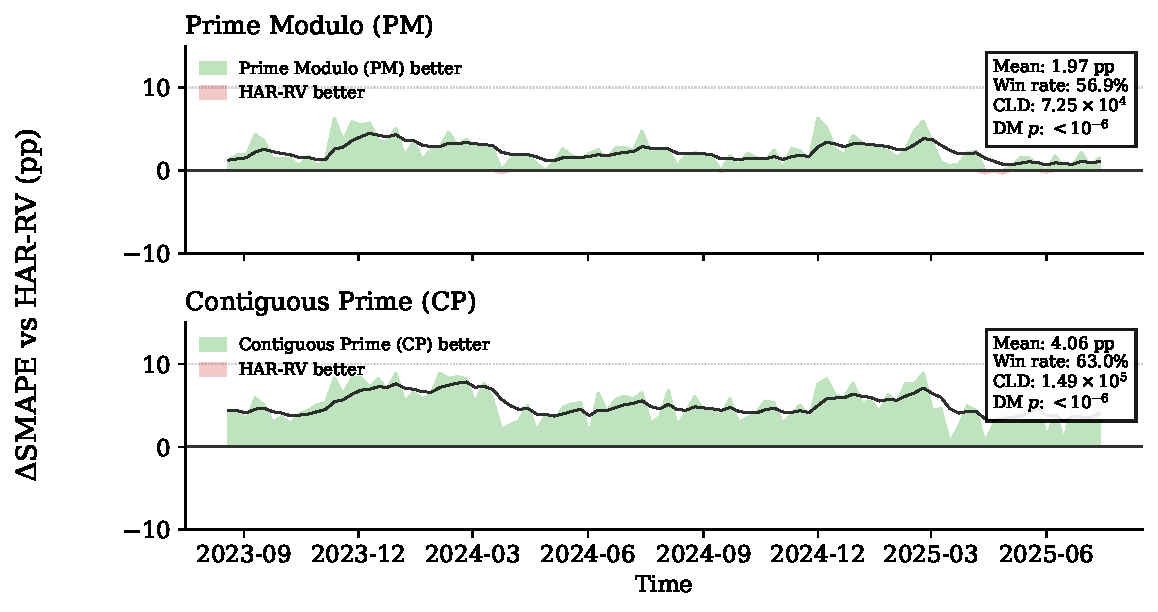
\includegraphics[width=0.94\textwidth]{paper_assets/figures/Section_4_fig_3_error_advantage_ALL_MEAN.pdf}
\captionof{figure}{SMAPE advantage relative to HAR-RV for the cross-sectional average series. Positive values indicate lower SMAPE for PM or CP. Shaded regions are weekly medians used for visual clarity, while the reported summary statistics are computed from the full-resolution series.}
\label{fig:error_advantage}
\end{center}}

\noindent
Figure~\ref{fig:error_advantage} clarifies how the aggregate gains are distributed through time. PM improves on HAR-RV by 1.97 percentage points in mean per-timestamp SMAPE advantage, with a 56.9\% timestamp win rate and a 2.04 percentage point median advantage. CP is materially stronger, with a 4.06 percentage point mean advantage, a 63.0\% timestamp win rate, and a 5.16 percentage point median advantage. For both models, the corresponding Diebold--Mariano tests reject equal predictive accuracy at $p < 10^{-6}$.

\noindent
The gain profile is also balanced rather than outlier-driven. When PM outperforms HAR-RV, the average gain is 9.85 percentage points, versus an 8.43 percentage point average loss when it does not. For CP, those figures are 13.07 and 11.28 percentage points respectively. That asymmetry, together with the positive timestamp win rates, indicates that the improvement arises from many recurrent advantages rather than from a small number of isolated episodes.

\subsection{Ablations and Drivers}

\noindent
The current \texttt{test\_7} paper bundle does not yet include a Section 5 package that is fully aligned with the ten-asset cross-sectional intraday evaluation used above. Figures 4 through 6 and Tables 3 and 4 are therefore omitted from the main draft rather than being populated with older, non-comparable outputs.

\noindent
Those ablations remain central to the final empirical argument because they separate three competing explanations for the observed gains: genuinely informative order structure, simple parameter expansion, and accidental feature enrichment. Once regenerated on the same ten-asset universe, Section 5 should establish whether the PM and CP gains survive controlled comparisons in capacity, modifiers, and randomized baselines.

\subsection{Statistical Significance by Asset Groups}

\noindent
The final question is where the gains are strongest. The broad pattern is that ordered features help most in large, liquid US equity exposures, remain positive but less precise in fixed income and international equity, and add little in commodities and metals.

{\renewcommand{\thefigure}{7}
\begin{center}

\includegraphics[width=0.88\textwidth]{paper_assets/figures/Section_6_fig_7_asset_groups.pdf}
\captionof{figure}{Average SMAPE improvement relative to HAR-RV by asset group.}
\label{fig:asset_groups}
\end{center}}

{\renewcommand{\thetable}{5}
\begin{center}
\captionof{table}{Group-level performance and significance by asset class. Positive $\Delta \mathrm{SMAPE}$ indicates lower SMAPE than HAR-RV.}
\label{tab:groups}
\small
\renewcommand{\arraystretch}{1.15}
\setlength{\tabcolsep}{8pt}
\begin{minipage}{0.88\textwidth}
\centering
\textbf{Panel A. Prime Modulo (PM)}\\[0.1cm]
\begin{tabular}{|l|c|c|c|}
\hline
Asset Group & $\Delta \mathrm{SMAPE}$ (pp) & Asset Win Rate (\%) & Fisher Combined $p$-value \\
\hline
US Mega Tech & 1.26 $\pm$ 0.13 & 100\% & $6.11 \times 10^{-33}$ \\
Broad US Equity & 1.51 $\pm$ 0.10 & 100\% & $6.30 \times 10^{-19}$ \\
International Equity & 0.13 $\pm$ 0.13 & 100\% & $< 10^{-300}$ \\
Commodities/Metals & -0.04 & 0\% & $9.75 \times 10^{-12}$ \\
Fixed Income & 0.31 $\pm$ 0.24 & 100\% & $< 10^{-300}$ \\
\hline
\end{tabular}
\end{minipage}

\vspace{0.25cm}

\begin{minipage}{0.88\textwidth}
\centering
\textbf{Panel B. Contiguous Prime (CP)}\\[0.1cm]
\begin{tabular}{|l|c|c|c|}
\hline
Asset Group & $\Delta \mathrm{SMAPE}$ (pp) & Asset Win Rate (\%) & Fisher Combined $p$-value \\
\hline
US Mega Tech & 1.79 $\pm$ 0.25 & 100\% & $< 10^{-300}$ \\
Broad US Equity & 2.99 $\pm$ 0.07 & 100\% & $< 10^{-300}$ \\
International Equity & 0.16 $\pm$ 0.34 & 50\% & $< 10^{-300}$ \\
Commodities/Metals & 0.04 & 100\% & $< 10^{-300}$ \\
Fixed Income & 0.59 $\pm$ 0.56 & 100\% & $< 10^{-300}$ \\
\hline
\end{tabular}
\end{minipage}

\vspace{0.1cm}
\footnotesize \parbox{0.92\textwidth}{\textit{Notes:} Asset Win Rate is the share of assets in each group with positive $\Delta \mathrm{SMAPE}$ relative to HAR-RV. Fisher combined $p$-values aggregate per-asset Diebold--Mariano tests based on absolute-error loss. Values below machine precision are reported as $< 10^{-300}$. Standard errors are unavailable for single-asset groups.}
\end{center}}

\noindent
Figure~\ref{fig:asset_groups} and Table~\ref{tab:groups} make the cross-sectional pattern explicit. The largest gains appear in Broad US Equity and US Mega Tech, where both PM and CP improve on every asset and where CP delivers the largest group-level gains. Fixed Income remains positive but is estimated less precisely, while International Equity is positive on average with wider dispersion. Commodities and Metals are essentially flat, with PM slightly negative and CP only marginally positive.

\noindent
This cross-group pattern is economically coherent. The strongest gains arise in deep, liquid equity exposures where intraday volatility clustering is persistent and ordered lag structure is likely to be informative. Markets that are more exposed to exogenous jumps or thinner intraday participation show much weaker benefits, which suggests that the value of the prime-based extensions depends on the extent to which short-run order carries stable information.


\section{Future Improvements}

...

\newpage
\appendix
\renewcommand{\thesection}{Appendix \Alph{section}}

\section{Daily Mirror of Overall Accuracy}

{\renewcommand{\thetable}{1B}
\begin{center}
\captionof{table}{Overall forecasting performance at the daily horizon. Lower values are better except for Directional Accuracy.}
\label{tab:overall_daily}
\small
\renewcommand{\arraystretch}{1.15}
\setlength{\tabcolsep}{6pt}
\begin{tabular}{|l|c|c|c|c|c|}
\hline
Model & SMAPE (\%) & \shortstack{RMSE\\$(\times 10^{-3})$} & \shortstack{MAE\\$(\times 10^{-3})$} & \shortstack{MedAE\\$(\times 10^{-3})$} & \shortstack{Directional\\Accuracy (\%)} \\
\hline
HAR-RV & \textbf{36.45 $\pm$ 2.46} & \textbf{7.515 $\pm$ 1.002} & \textbf{4.467 $\pm$ 0.527} & \textbf{3.069 $\pm$ 0.354} & \textbf{70.06 $\pm$ 0.69} \\
Prime Modulo (PM) & 37.64 $\pm$ 2.37 & 7.649 $\pm$ 1.014 & 4.640 $\pm$ 0.560 & 3.114 $\pm$ 0.366 & 68.69 $\pm$ 0.89 \\
Contiguous Prime (CP) & 37.88 $\pm$ 2.40 & 7.744 $\pm$ 1.016 & 4.705 $\pm$ 0.569 & 3.121 $\pm$ 0.369 & 69.35 $\pm$ 0.85 \\
\hline
\end{tabular}

\vspace{0.1cm}
\footnotesize \parbox{0.92\textwidth}{\textit{Notes:} Entries report the cross-sectional mean with standard errors across assets. Error columns are rescaled for readability. Each asset contributes roughly 396 aligned daily observations. Bold marks the best value in each column.}
\end{center}}

\noindent
Table~\ref{tab:overall_daily} is included as a supporting appendix result rather than a main-text finding. On this daily sample, HAR-RV has the lowest average SMAPE, RMSE, MAE, and MedAE, while PM and CP do not preserve the intraday ordering seen in Table~\ref{tab:overall_intraday}. The daily mirror therefore places a clear boundary on the main empirical claim of the paper: the present advantage of the prime-based extensions is concentrated at the intraday horizon rather than being a uniform improvement across sampling frequencies.

\section{Metric Definitions and Inference}

\noindent
Let $y_{i,t}$ denote the realized volatility for asset $i$ at evaluation time $t$, and let $\hat{y}^{\,m}_{i,t}$ denote the forecast from model $m$. Define the forecast error $e^{\,m}_{i,t} = y_{i,t} - \hat{y}^{\,m}_{i,t}$. All main-text tables first compute metrics at the asset level and then average those asset-level quantities across the cross-section.

\vspace{0.15cm}
\noindent \textbf{Forecast metrics.}
For an asset with $T_i$ aligned evaluation observations, the reported metrics are
\begin{align*}
\mathrm{SMAPE}^{\,m}_i &= \frac{200}{T_i}\sum_{t=1}^{T_i}\frac{|y_{i,t}-\hat{y}^{\,m}_{i,t}|}{|y_{i,t}|+|\hat{y}^{\,m}_{i,t}|},\\
\mathrm{RMSE}^{\,m}_i &= \sqrt{\frac{1}{T_i}\sum_{t=1}^{T_i}\left(e^{\,m}_{i,t}\right)^2},\\
\mathrm{MAE}^{\,m}_i &= \frac{1}{T_i}\sum_{t=1}^{T_i}\left|e^{\,m}_{i,t}\right|,\\
\mathrm{MedAE}^{\,m}_i &= \mathrm{median}_{1 \leq t \leq T_i}\left|e^{\,m}_{i,t}\right|.
\end{align*}
Directional Accuracy is computed from the sign of the realized next-step change relative to the sign implied by the forecast:
\begin{align*}
\mathrm{DA}^{\,m}_i
= \frac{100}{T_i-1}\sum_{t=2}^{T_i}
\mathbf{1}\!\left\{
\mathrm{sign}(y_{i,t}-y_{i,t-1})
=
\mathrm{sign}(\hat{y}^{\,m}_{i,t}-y_{i,t-1})
\right\}.
\end{align*}

\vspace{0.15cm}
\noindent \textbf{Cross-sectional aggregation.}
If $M_i^{\,m}$ denotes any one of the asset-level metrics above, the tables report
\begin{align*}
\bar{M}^{\,m} &= \frac{1}{N}\sum_{i=1}^{N} M_i^{\,m},\\
\mathrm{SE}\!\left(\bar{M}^{\,m}\right) &= \frac{s(M_1^{\,m},\ldots,M_N^{\,m})}{\sqrt{N}},
\end{align*}
where $N$ is the number of assets and $s(\cdot)$ is the sample standard deviation across assets.

\vspace{0.15cm}
\noindent \textbf{Advantage measures used in Figures 3 and 7 and in Table 5.}
For the timestamp-level advantage plot, we define
\begin{align*}
\delta_t^{\,m}
=
\mathrm{SMAPE}_{\mathrm{HAR},t}
-
\mathrm{SMAPE}_{m,t},
\end{align*}
so positive values indicate that model $m$ improves on HAR-RV at time $t$. The summary statistics in Figure~\ref{fig:error_advantage} are then based on the full-resolution sequence $\{\delta_t^{\,m}\}$:
\begin{align*}
\overline{\delta}^{\,m} &= \frac{1}{T}\sum_{t=1}^{T}\delta_t^{\,m},\\
\mathrm{WinRate}^{\,m}_{\mathrm{time}} &= \frac{100}{T}\sum_{t=1}^{T}\mathbf{1}\{\delta_t^{\,m}>0\},\\
\mathrm{CLD}^{\,m} &= \sum_{t=1}^{T}\delta_t^{\,m}.
\end{align*}
For the asset-group analysis, the relevant object is the asset-level improvement
\begin{align*}
\Delta \mathrm{SMAPE}^{\,m}_i
=
\mathrm{SMAPE}^{\,\mathrm{HAR}}_i
-
\mathrm{SMAPE}^{\,m}_i,
\end{align*}
which is averaged within each group $g$ as
\begin{align*}
\overline{\Delta \mathrm{SMAPE}}^{\,m}_g
=
\frac{1}{N_g}\sum_{i \in g}\Delta \mathrm{SMAPE}^{\,m}_i,
\qquad
\mathrm{WinRate}^{\,m}_g
=
\frac{100}{N_g}\sum_{i \in g}\mathbf{1}\{\Delta \mathrm{SMAPE}^{\,m}_i>0\}.
\end{align*}
Accordingly, the win rate in Figure~\ref{fig:error_advantage} is a timestamp-level quantity, whereas the win rates in Table~\ref{tab:groups} are asset-level quantities.

\vspace{0.15cm}
\noindent \textbf{Diebold--Mariano and Fisher combined inference.}
For a given loss function $L(\cdot)$, the asset-level Diebold--Mariano test is built from the loss differential
\begin{align*}
d^{\,m}_{i,t}
=
L\!\left(e^{\,\mathrm{HAR}}_{i,t}\right)
-
L\!\left(e^{\,m}_{i,t}\right),
\end{align*}
with statistic
\begin{align*}
\mathrm{DM}^{\,m}_i
=
\frac{\bar{d}^{\,m}_i}{\sqrt{\widehat{\mathrm{Var}}_{\mathrm{NW}}(\bar{d}^{\,m}_i)}}.
\end{align*}
Figure~\ref{fig:error_advantage} applies this logic to the timestamp-level SMAPE differential, while Table~\ref{tab:groups} combines per-asset Diebold--Mariano $p$-values based on absolute-error loss. If $\{p^{\,m}_{i,g}\}_{i \in g}$ are the valid per-asset $p$-values for group $g$, the Fisher combined statistic is
\begin{align*}
X^{\,m}_g &= -2\sum_{i \in g}\log p^{\,m}_{i,g},\\
p^{\,m,\mathrm{Fisher}}_g &= 1 - F_{\chi^2_{2N_g}}\!\left(X^{\,m}_g\right),
\end{align*}
where $F_{\chi^2_{2N_g}}$ is the chi-squared cumulative distribution function with $2N_g$ degrees of freedom.


\begin{thebibliography}{1} % 1 = Number of items
\bibitem{1} Insert citation for HAR-RV paper by Yue Zhao.


\end{thebibliography}

\end{document}
